
\begin{figure}
  \caption{The cost curves for the real-world datasets.}
  \label{fig:cost-curves-real-world-datasets}
  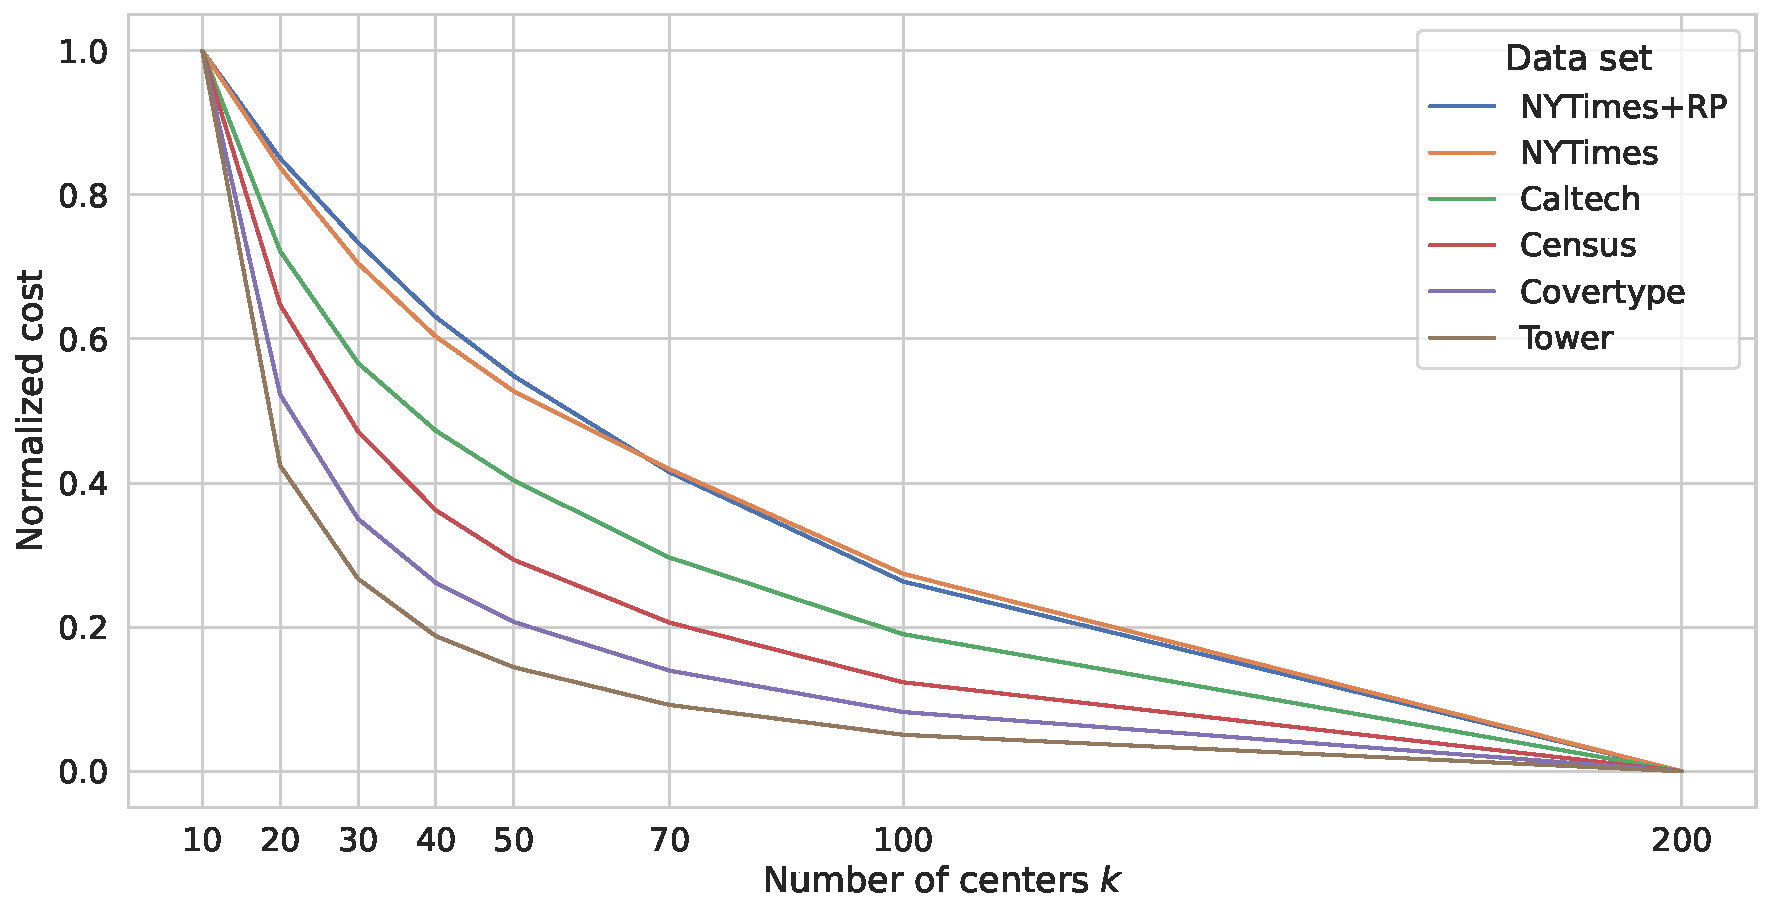
\includegraphics[width=1\linewidth]{figures/cost-curves-real-world-datasets.pdf}
\end{figure}


\begin{figure}
  \caption{The cost curves for the benchmark.}
  \label{fig:cost-curves-benchmark}
  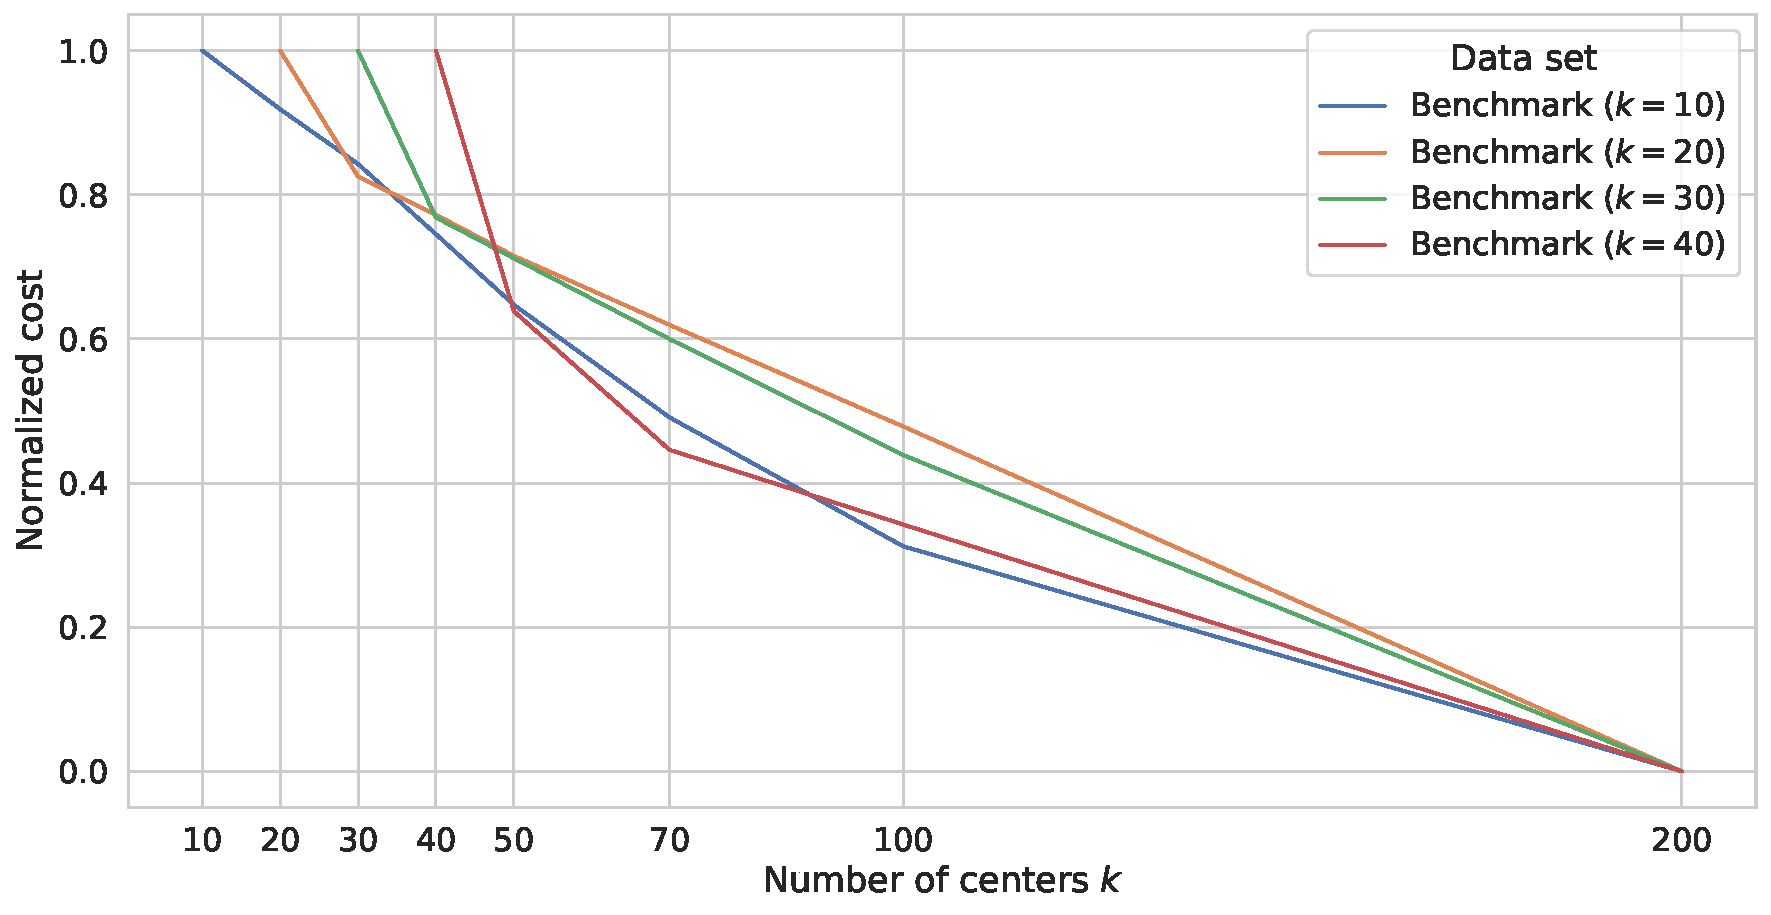
\includegraphics[width=1\linewidth]{figures/cost-curves-benchmark.pdf}
\end{figure}


\section{Experiments} \label{sec:experiments}
% Describe the "what": coresets vs optimization. What are we doing? What do we expect?
In this section, we present an empirical evaluation of $k$-means coreset constructions.
The outperformance of a coreset algorithm cannot be fully determined by the outcome of an optimization after the coreset is generated because a coreset algorithm may ultimately yield a good clustering yet fail to produce a high quality coreset with low distortion.
% The full picture of which coreset algorithm is best may not be revealed if one simply evaluate coreset algorithms by comparing the best possible clustering in terms of the lowest cost.
Therefore, departing from other works which evaluate coreset algorithms based on the output of an optimization algorithm, we instead separate the task of computing a coreset from the optimization task and evaluate the quality of coresets in isolation. 

% Why benchmark? Because it is certain to be different from optimization.
It is worthwhile to evaluate coresets on a synthetic data for two reasons. First, it is easier to make a fair evaluation if the synthetic data is known to generate hard instances for any coreset algorithm. Second, the evaluation procedure can consider both good and bad clusterings as they will be known beforehand. These two points are not always clear for real-world data sets.

% Issues with real-world data sets.
For real-world data sets, it is not uncommon to observe that $k$-means cost to drop significantly for larger values of $k$. ~\cref{fig:cost-curves-real-world-datasets} illustrate this behavior for several real-world datasets. The more the curve bends, the less of a difference there is between computing a coreset and a clustering with low cost. In this case, a coreset algorithm adding more centers to the coreset will seem to be performing well when evaluating it based on the outcome of the optimization. However, in the benchmark dataset, there is no way to reduce the cost without capturing the right subclusters within the instance. This means that the cost does not decrease markedly beyond a certain value of $k$ even if more centers are added as seen in~\cref{fig:cost-curves-benchmark}. In this work, we nevertheless study real-world data sets to determine whether the difference between coresets and optimization can be observed in these data sets.




% Describe how we measure distortion.
For estimating the quality of the coresets produced by various coreset algorithms, we computed the distortions on real-world data sets and on the benchmark. On each real-world data set $A$, we first computed a coreset $\Omega$ and then ran $k$-means++ on $\Omega$ to find a set of $k$ centers $\calS$. The $k$-means++ algorithm was repeated 5 times in order to pick the set of centers with the lowest cost on $\Omega$.
\omar{While writing this, I checked the code and saw that it is picking a set of $k$ centers with the lowest cost! Is this wrong? Should I instead let $k$-means++ generate 5 sets of centers $\calS_1, \calS_2, \cdots, \calS_5$ and then pick the one with largest distortion?}
Afterwards, we computed the distortion
\begin{align*}
    \max\left(
      \frac{\cost_A(\calS)}{\cost_{\Omega}(\calS)},
      \frac{\cost_{\Omega}(\calS)}{\cost_A(\calS)}
    \right)
\end{align*}
For the benchmark, we computed the distortion following the evaluation procedure described in~\cref{sec:benchmark}. This experiment was repeated for each coreset algorithm $10$ times. We aggregated the reported distortions by taking the maximum over all $10$ evaluations. In addition, we also preprocessed the data using the dimension reduction techniques described in Section~\ref{sec:algorithms}.



% We now present the empirical evaluation of these coresets.
% We ran two kinds of experiments. On real-world data sets, we merely computed a coreset $\Omega$, followed by running $k$-means++ on $\Omega$. 
% The $k$-means++ algorithm was repeated 5 times, each yielding a solution $\calS_i$, and as the best lower bound on the distortion we used the largest ratio $\max_i\left(\max\left(\frac{\cost_A(\calS_i)}{\cost_{\Omega}(\calS_i)},\frac{\cost_{\Omega}(\calS_i)}{\cost_A(\calS_i)}\right)\right)$.
% For the benchmark, we used the evaluation as proposed in Section~\ref{sec:benchmark}. In addition, we also determined the distortion via simply running the $k$-means++ algorithm. 

% Except for BICO, which is deterministic, this experiment was repeated for each coreset algorithm $10$ times. \omar{Experiments were repeated 10 times including BICO. Although vanilla BICO is deterministic, we used BICO with heuristic speed optimizations which are stochastic.} We aggregated the reported distortions by taking the maximum over all $10$ evaluations. In addition, we also preprocessed the data using the dimension reduction techniques described in Section~\ref{sec:algorithms}.


\subsection{Datasets}
To evaluate the behavior of different algorithms, we conducted experiments on 5 real-world datasets, as shown in~\cref{tab:real-world-datasets-overview}, in addition to our proposed benchmark.

% The real-world datasets include
% \textit{Census}\footnote{\url{https://archive.ics.uci.edu/ml/datasets/US+Census+Data+(1990)}},
% \textit{Covertype}\footnote{\url{https://archive.ics.uci.edu/ml/datasets/covertype}}, and 
% \textit{Tower}\footnote{\url{http://homepages.uni-paderborn.de/frahling/coremeans.html}}
% ---
% and several instances of the proposed benchmark.

The \textit{Census}\footnote{\url{https://archive.ics.uci.edu/ml/datasets/US+Census+Data+(1990)}} dataset is a small subset of the Public Use Microdata Samples from 1990 US census. It consists of demographic information encoded as 68 categorical attributes of 2,458,285 individuals. 

\textit{Covertype}\footnote{\url{https://archive.ics.uci.edu/ml/datasets/covertype}} is comprised of cartographic descriptions and forest cover type of four wilderness areas in the Roosevelt National Forest of Northern Colorado in the US. It consists of 581,012 records, 54 cartographic variables and one class variable. Although \textit{Covertype} was originally made for classification tasks, it is often used for clustering tasks by removing the class variable~\cite{AckermannMRSLS12}.

\textit{Tower}\footnote{\url{http://homepages.uni-paderborn.de/frahling/coremeans.html}} is a 2,560 by 1,920 picture of a tower on a hill where each pixel is represented by a RGB color value. This dataset consists of 4,915,200 rows and 3 columns. 
We used the datasets \textit{Census}, \textit{Covertype} and \textit{Tower} as these are often used to evaluate the performance of coreset algorithms. 

To include larger datasets in evaluation, we used \textit{Caltech} and \textit{NYTimes}. \textit{Caltech} was inspired by~\cite{FGSSS13}. It was created by computing SIFT features from the images in the Caltech101 dataset\footnote{\url{http://www.vision.caltech.edu/Image_Datasets/Caltech101/}}. This database contains pictures of objects partitioned into 101 categories. Disregarding the categories, we concatenated the 128-dimensional SIFT vectors from each image into one large data matrix. 
We decided to include the \textit{NYTimes}\footnote{\url{https://archive.ics.uci.edu/ml/datasets/bag+of+words}} dataset in our experiments as the number of dimensions is very large. \textit{NYTimes} is composed of the word counts of 300,000 news articles from The New York Times. The vocabulary size of the text collection is 102,660.

To understand how denoising effects the quality of the coreset outputs, we applied Principal Component Analysis (PCA) on \textit{Caltech}, \textit{Census} and \textit{Covertype} by computing the $k$ singular vectors corresponding to the largest singular values. For these three datasets, we preserve the dimensions of the original datasets. For the \textit{NYTimes} dataset, we experimented with both PCA and terminal embeddings to reduce the number of dimensions.

As for the benchmark dataset, instances were generated to roughly match the sizes of the real-world datasets. The chosen parameters values and the corresponding dataset sizes are shown in ~\cref{tab:benchmark-instances-overview}. 
% We generated a set of instances with no scaling i.e., $\beta=1.0$ (referred to as \textit{Benchmark-1.0}) and with maximum scaling; $\beta = 2.0$ (\textit{Benchmark-2.0}).




%
\begin{table}
	\begin{center}%\centering
	\caption{The sizes of the real-world datasets used for the experimental evaluation}
	\label{tab:real-world-datasets-overview}
% 	\resizebox{\textwidth}{!}{
	\begin{tabular}{lrr}
		\toprule
        
		    & Data points
		    & Dimensions
            \\
		\midrule
		\textit{Caltech}
    		& 3,680,458
    		& 128
    		\\
		\textit{Census}
    		& 2,458,285
    		& 68
    		\\
	    \textit{Covertype}
    	    & 581,012
    		& 54
    		\\
	    \textit{NYTimes}
    	    & 500,000
    		& 102,660
    		\\
        \textit{Tower}
            & 4,915,200
    		& 3
    		\\
		\bottomrule
	\end{tabular}\\
	\end{center}
% 	}
\end{table}



%
\begin{table}
	\begin{center}%\centering
	\caption{The parameter values and the sizes of the benchmark instances used for the experimental evaluation.}
	\label{tab:benchmark-instances-overview}
% 	\resizebox{\textwidth}{!}{
	\begin{tabular}{rrrr}
		\toprule
        $k$
		    & $\alpha$
		    & Data points
		    & Dimensions
            \\
		\midrule
        10
    		& 6
    		& 1,000,000
    		& 60
    		\\
        20
    		& 5
    		& 3,200,000
    		& 100
    		\\
        30
    		& 4
    		& 810,000
    		& 120
    		\\
        40
    		& 4
    		& 2,560,000
    		& 160
    		\\
    %     50
    % 		& 4
    % 		& 6,250,000
    % 		& 200
    % 		\\
		\bottomrule
	\end{tabular}\\
	\end{center}
% 	}
\end{table}

\subsection{Algorithm Parameters}
We followed the same experimental procedure with respect to the choice of parameter values for the algorithms as prior works~\cite{AckermannMRSLS12, FGSSS13}. For the target coreset size, we used $200k$ for all our experiments. On \textit{Caltech}, \textit{Census},  \textit{Covertype} and \textit{NYTimes}, we used $k$ values in $\{10, 20, 30, 40, 50\}$, while for \textit{Tower} we used larger cluster sizes $k \in \{20, 40, 60, 80, 100\}$. On the benchmark instances, we settled on $k \in \{10, 20, 30, 40\}$ as a reasonable trade-off between running time and dataset size.



\subsection{Setup}
We implemented Sensitivity Sampling, Group Sampling, Ray Maker, and StreamKM++ in C++. The source code can be found on GitHub\footnote{Link to repository will be provided later.}. For BICO, we used the authors' reference implementation\footnote{\url{https://ls2-www.cs.tu-dortmund.de/grav/en/bico}}. The source code was compiled with gcc 9.3.0. The experiments were performed on a machine with 14 cores (3.3 GHz) and 256 GB of memory.

\subsection{Results}

\begin{figure*}
  \caption{The distortions of the evaluated algorithms on 5 real-world datasets and on the proposed benchmark. Lower bar is better.}
  \label{fig:distortions}
  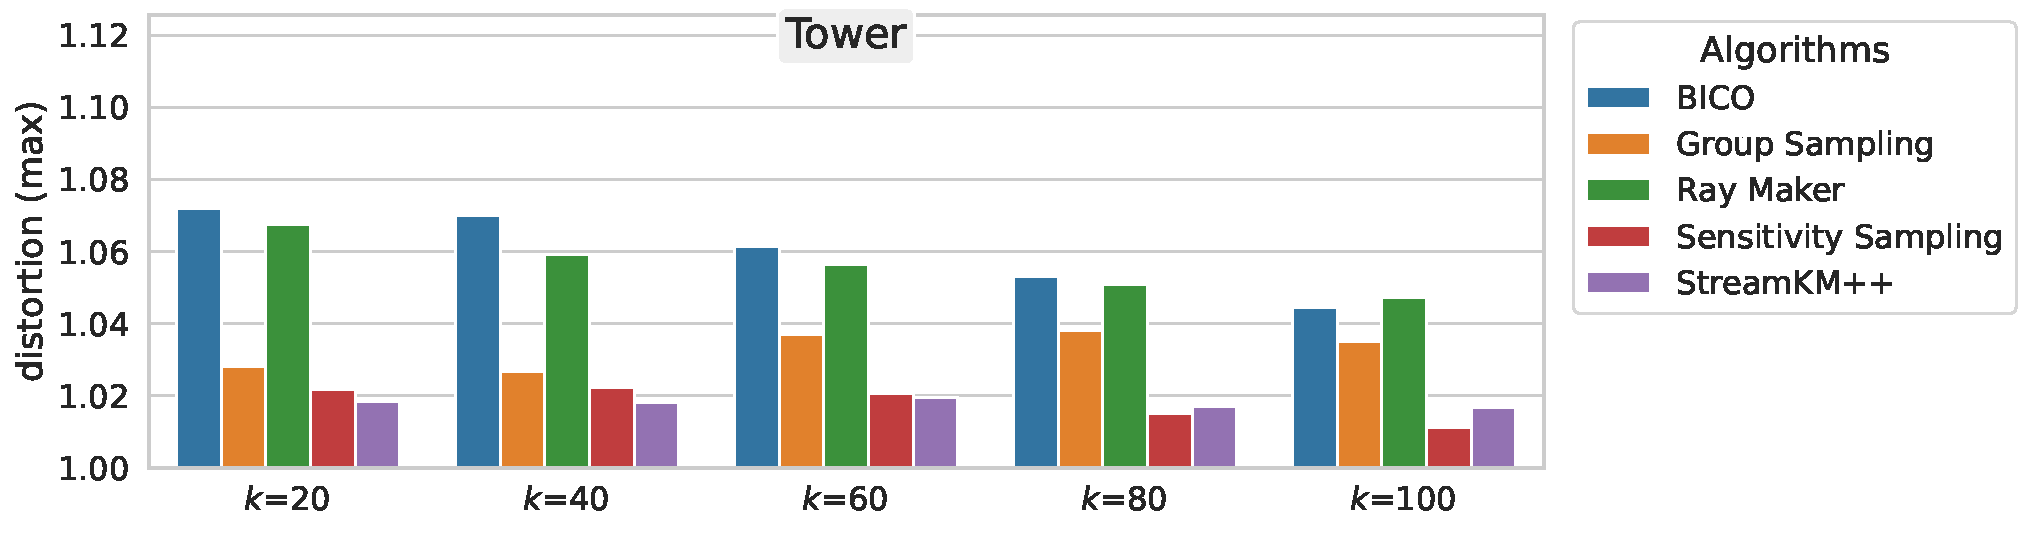
\includegraphics[width=.65\linewidth]{figures/distortions-Tower.pdf}
  \newline \newline
  \subfloat{
    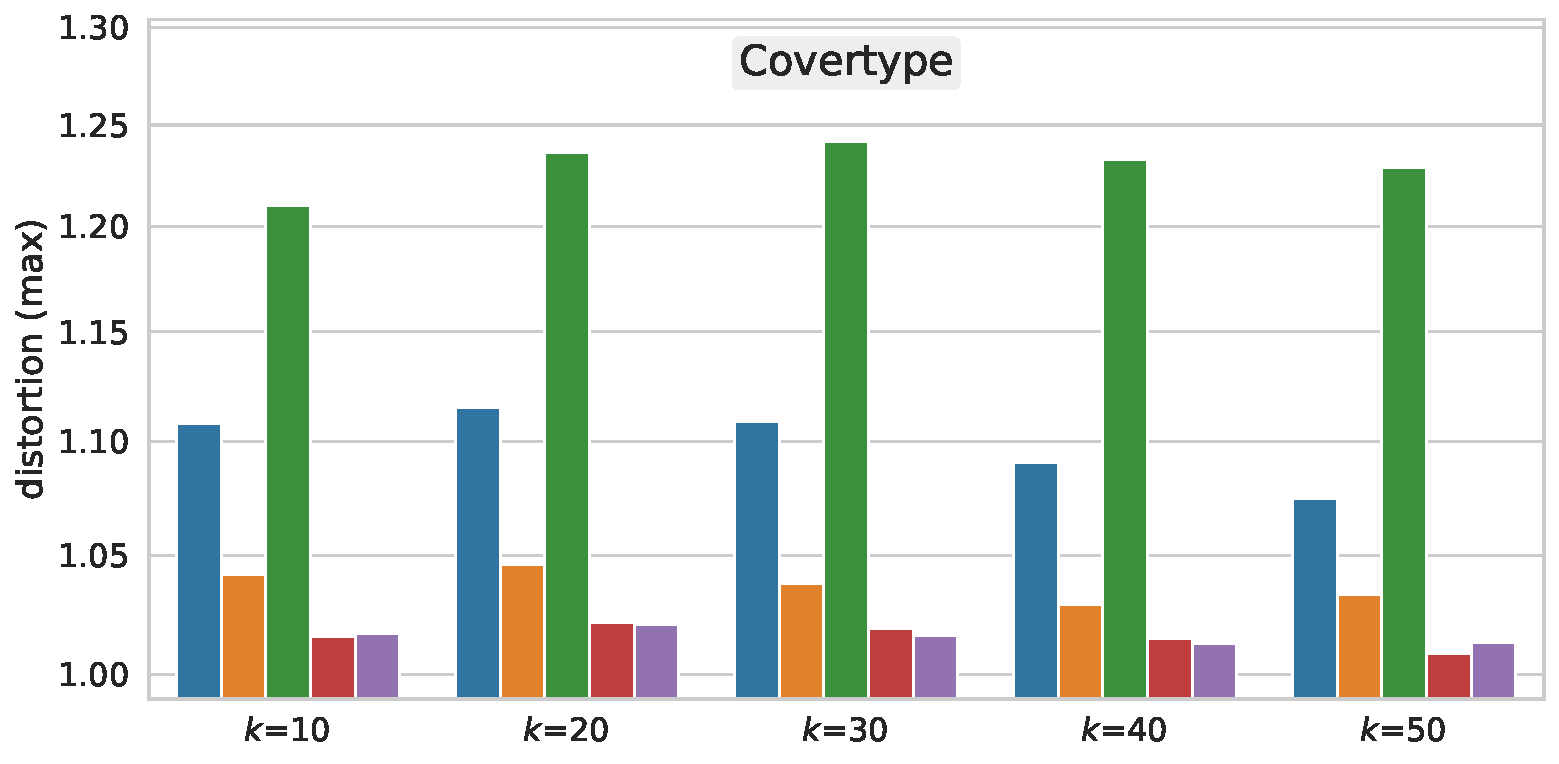
\includegraphics[width=0.5\textwidth]{figures/distortions-Covertype.pdf}
  }
  \subfloat{
    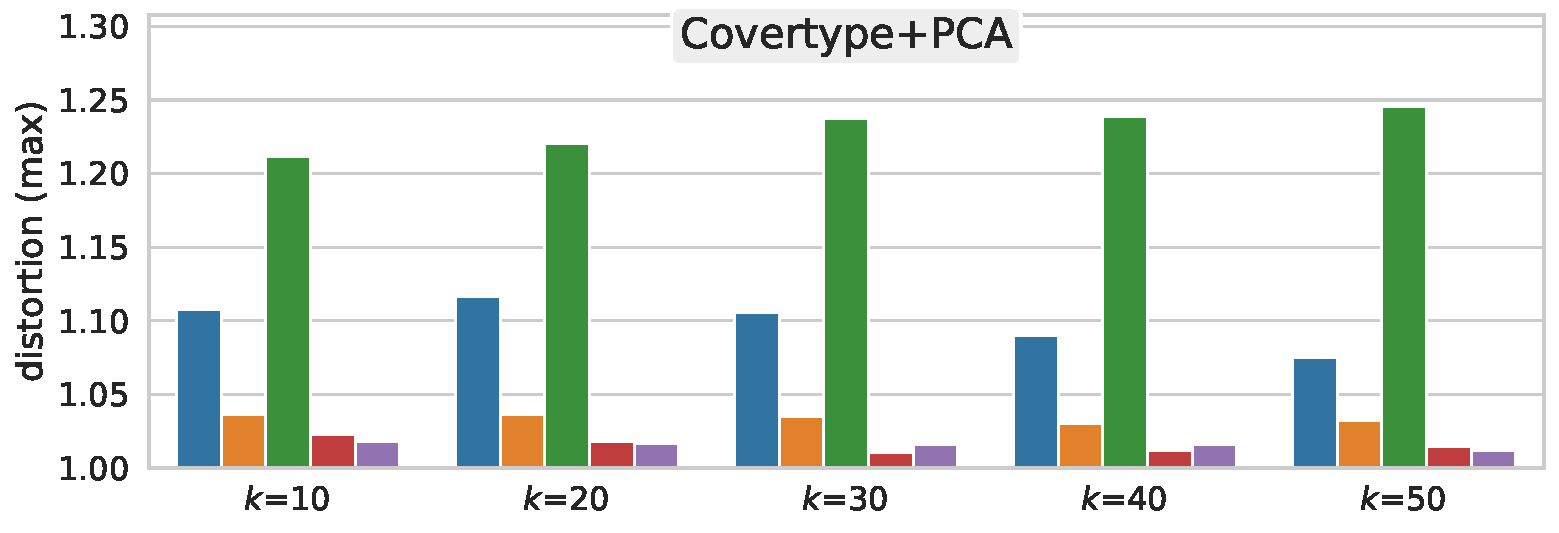
\includegraphics[width=.5\linewidth]{figures/distortions-Covertype+PCA.pdf}
  }
  \newline \newline
  \subfloat{
    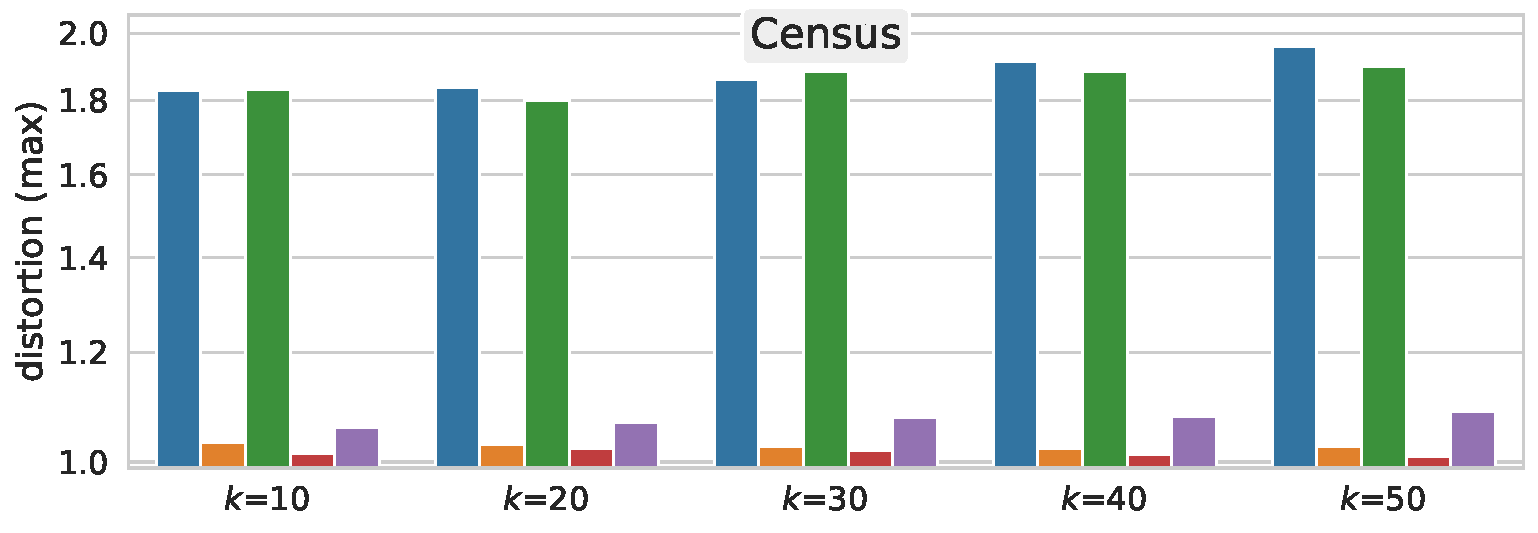
\includegraphics[width=0.5\textwidth]{figures/distortions-Census.pdf}
  }
  \subfloat{
    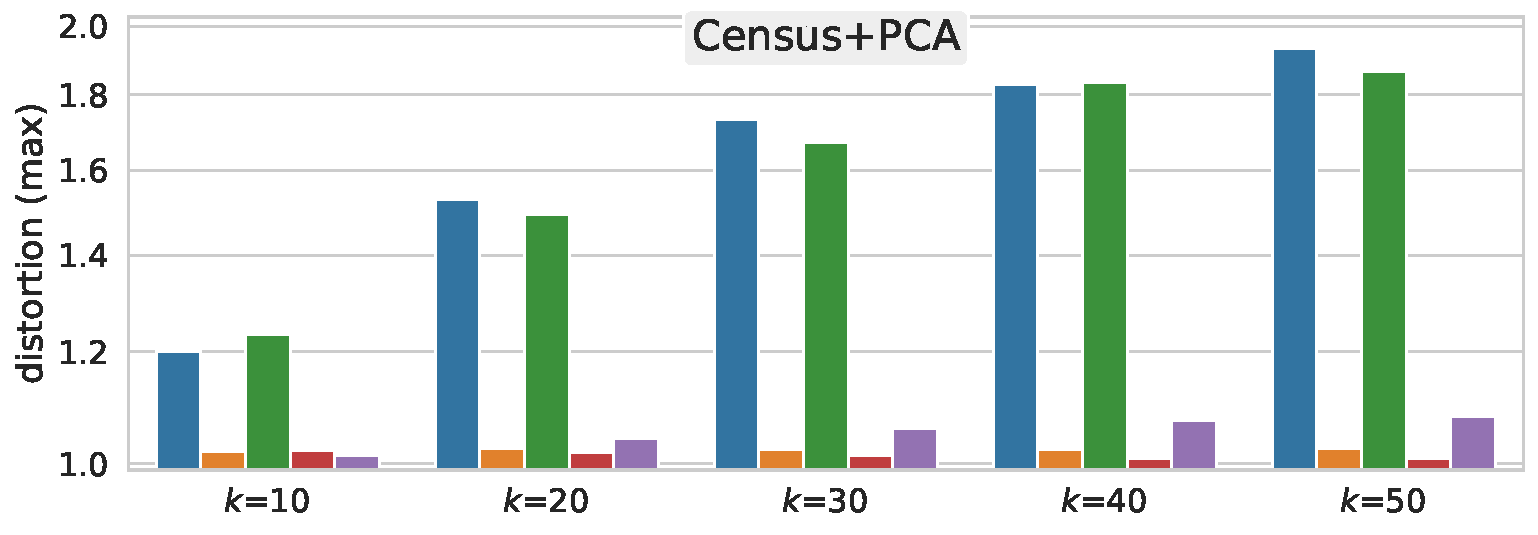
\includegraphics[width=.5\linewidth]{figures/distortions-Census+PCA.pdf}
  }
  \newline \newline
  \subfloat{
    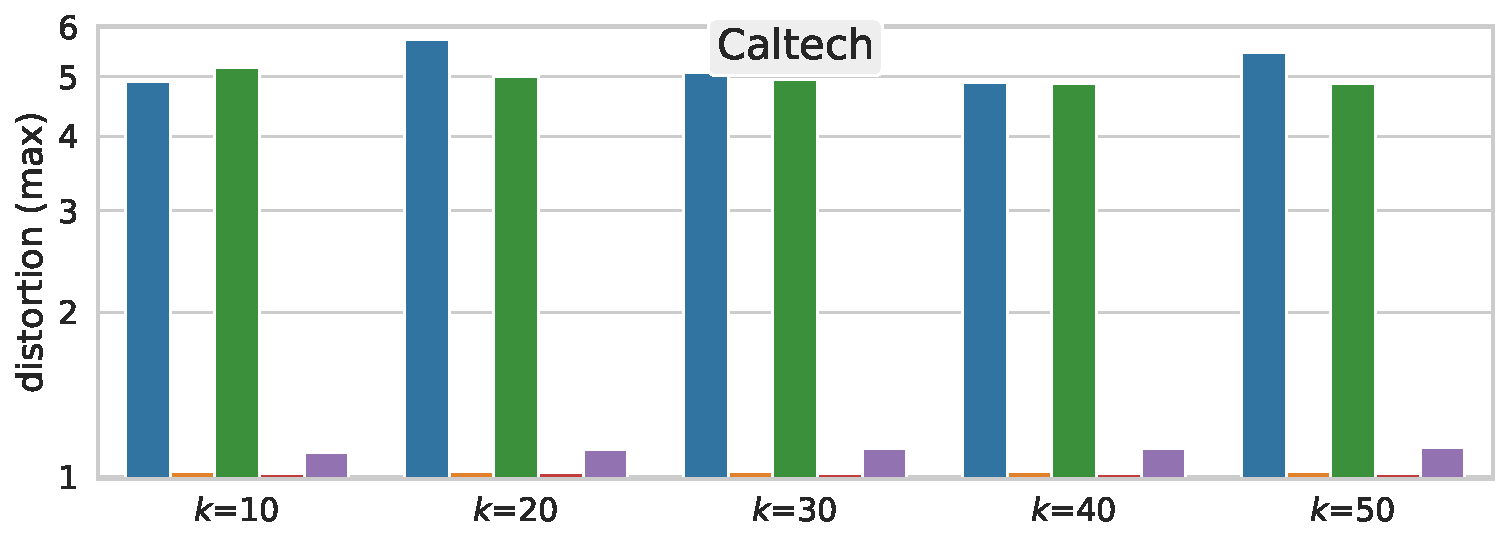
\includegraphics[width=0.5\textwidth]{figures/distortions-Caltech.pdf}
  }
  \subfloat{
    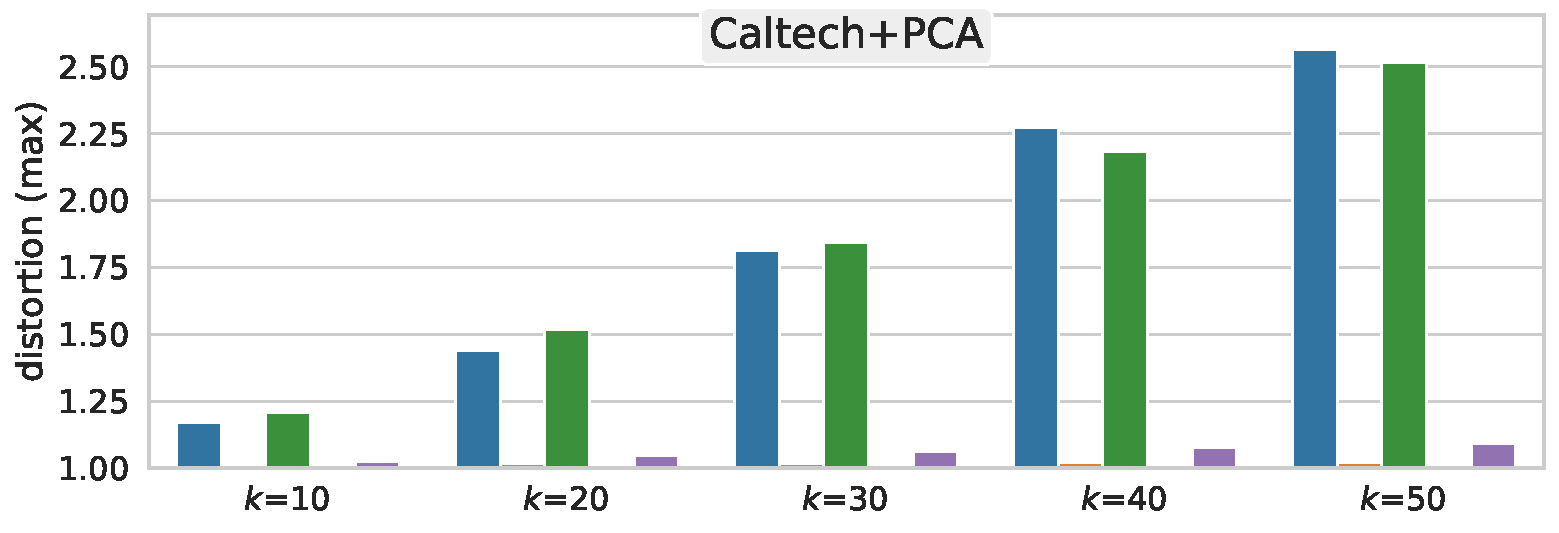
\includegraphics[width=.5\linewidth]{figures/distortions-Caltech+PCA.pdf}
  }
  \newline \newline
  \subfloat{
    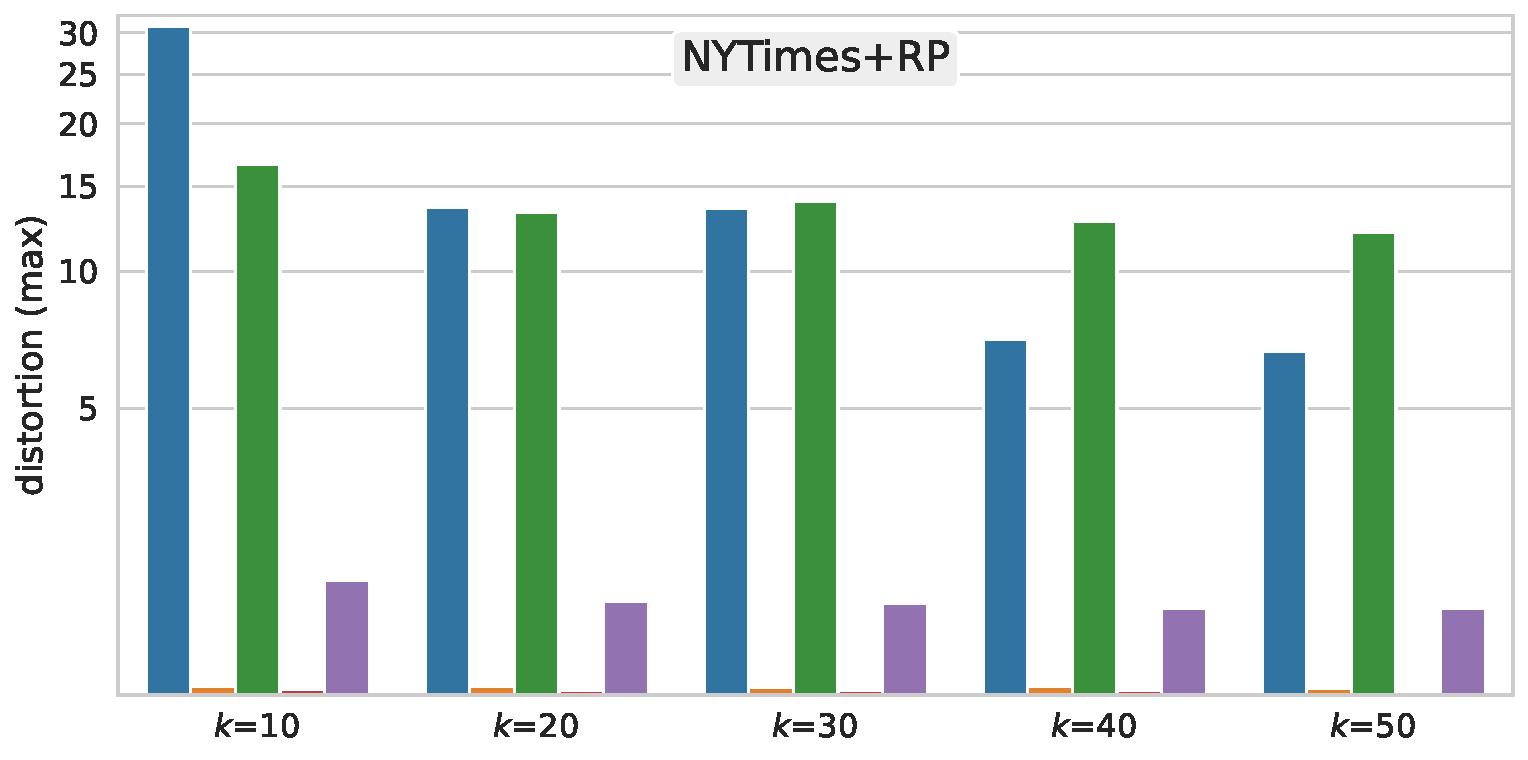
\includegraphics[width=0.5\textwidth]{figures/distortions-NYTimes+RP.pdf}
  }
  \subfloat{
    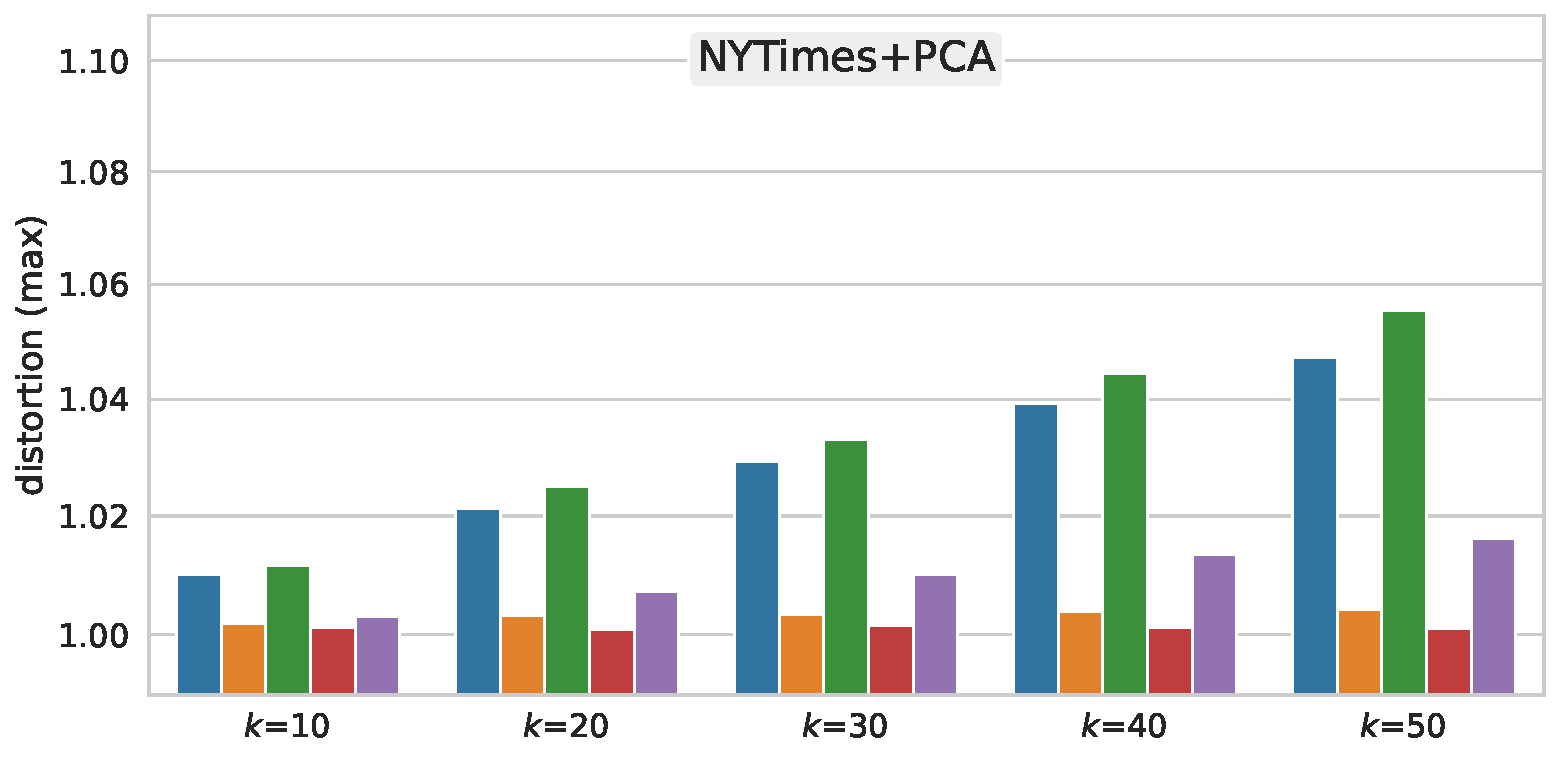
\includegraphics[width=.5\linewidth]{figures/distortions-NYTimes+PCA.pdf}
  }
  \newline \newline
  \subfloat{
    \\[1ex]
    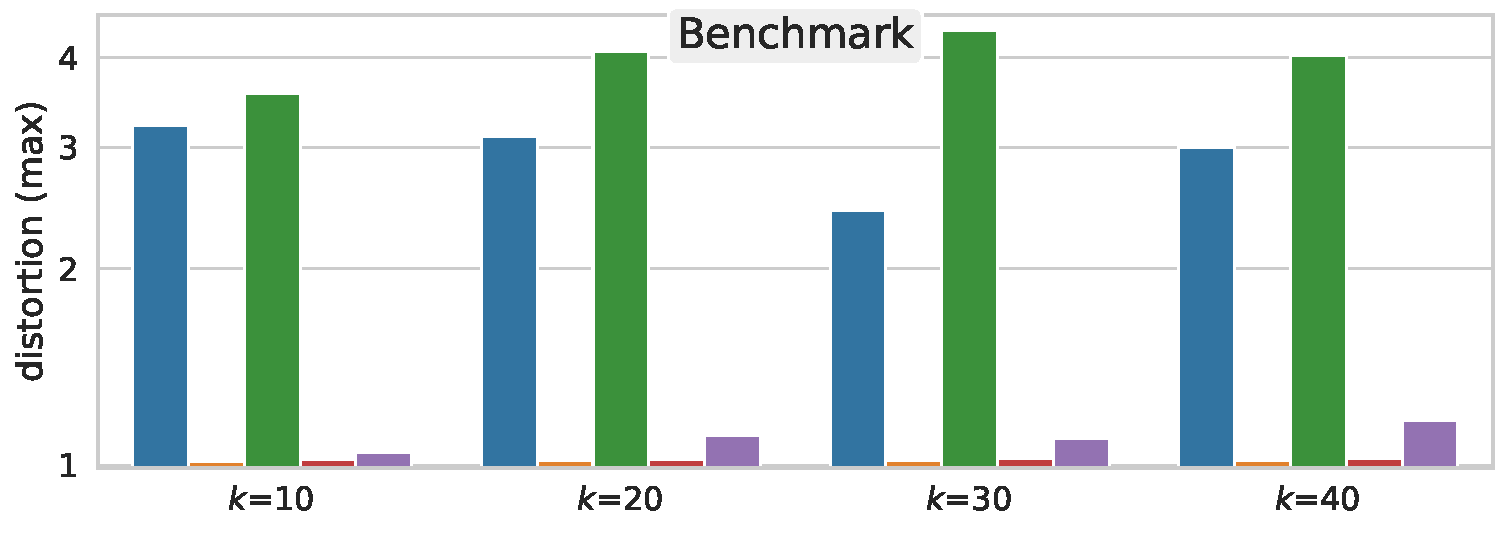
\includegraphics[width=0.5\textwidth]{figures/distortions-Benchmark.pdf}
  }
  \subfloat{
    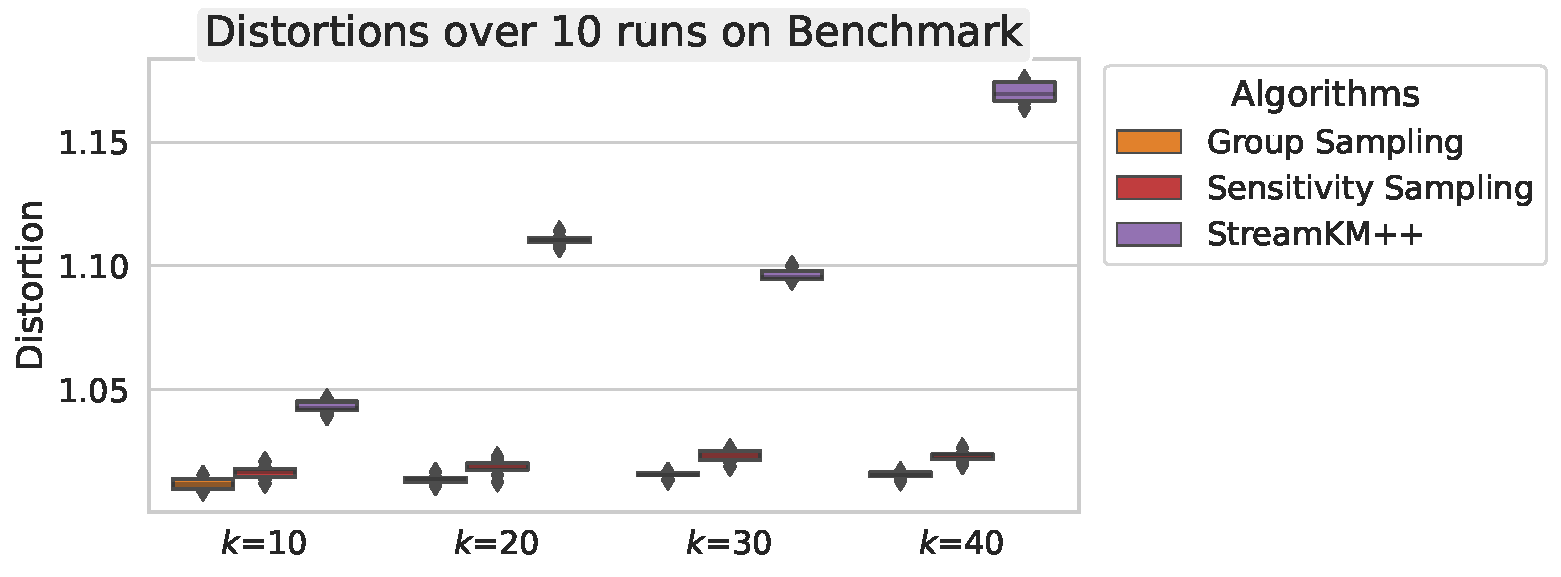
\includegraphics[width=.5\linewidth]{figures/boxplot-Benchmark-GS-SS-StreamKM.pdf}
  }
  
\end{figure*}

We summarized the results in \cref{fig:distortions}.
All five algorithms are matched on the \textit{Tower} dataset. The worst distortions across the algorithms are close to 1, and performance between the algorithms is negligible. \textit{Tower} is a simple dataset with very low dimensionality ($d=3$). The performance difference between sampling-based and movement-based methods become more pronounced as the number of dimensions increase. On \textit{Covertype} with its 54 features, Ray Maker performs the worst followed by BICO. The performance does not change much despite reducing noise with PCA. Differences in performance are more stark on \textit{Census} and \textit{Caltech} where methods based on importance sampling are better. For \textit{Census} ($d=68$), the preprocessing step with PCA improves the performance of BICO and Ray Maker slightly for lower values of $k$. The distortions of BICO and Ray Maker are reduced markedly on \textit{Caltech} ($d=128$) after applying PCA. We observe that BICO and Ray Maker have very large distortions on \textit{NYTimes} when random projections are used for dimensionality reduction. On the \textit{Benchmark} dataset, Ray Maker is the worst while Sensitivty Sampling and Group Sampling are the best. StreamKM++ performs also very well compared to BICO.
